\chapter{Diffusion and discussion of results}

This chapter aims to summarize the results of this thesis and to critically discuss them.
Furthermore, the results should be set into perspective with literature to better emphasize the potential
and make the reuslts comparable. 
Wherever possible a generalization of results should be established.

\section{Solution architecture and Hyperparameter tuning}

The first result is the developed \ac{IT}-artifact\ref{Overall architecture} as overall solution architecture. 
The required components for the combination of the digital computer with the \ac{mem-HNN} accelerator 
is universally valid and can be used to train Boltzmann Machines with the Hopfield Neural Network as sampling method. 
This is validated by the successful \ac{DSR} outcomes which proved the possibility of efficiently 
training a Boltzmann Machine with a good prediction accuracy.
Despite, the training is done by a simulation and not done on the actual \ac{mem-HNN}, which can be seeen as critics 
all the calculations and hardware components are correctly mapped in the software and are validated by each iterative design and evaluation phase.
Furthermore, this procedure is part of the \ac{ASIC} design process before building and using the physical accelerator.

In an next step the baselines for the training are established using Gibbs sampling and Metropolis Hastings.
\textbf{Gibbs Sampling} is the most \textbf{sensitive} method with an prediction accuracy of \(\mathbf{92.29\%}\), while
\textbf{Metropolis Hastings} is far more stable with a faster learning curve and an total prediction accuracy of \(\mathbf{94.15\%}\).
After setting these Baselines, the implementation of the noisy injected Hopfield Network is achieved, which is the main result for the thesis. 
Continuation of known proof of concepts, a full training for the noise injected Hopfield Network is done by adding a random gaussian distribution 
to the activation function of the \ac{RBM} shown in \ref{Noisy_acitivation_function_good}. 
First, the metric predition accuracy is of interest, since this helps to compare with the other two conventional sampling methods and preferably surpasses them.

Hence, the \textbf{asynchronously Hopfield Network} achieved an baseline of \(\mathbf{90.81\%}\) without Hyperparameter tuning but has a more stable  learning rate than Gibbs Sampling and
is equal with Metropolis Hastings.
Here, the Hyperparameter tuning can be highlighted since until now there was no data available for such an \ac{IT}-artifact and especially not for the Hopfield Network sampling method.
With some adjustments made to the scale, which represents the standard deviation of the injected noise the stability, the performance is meassured.
The outcome is at an scale of 1.6 the prediction accuracy is the highest of all with a value of \(\mathbf{94.77\%}\) shown in \ref{Hyperparamers_Scale_ohne}.
In comparison, the \textbf{N/2 Half Hopfield Network} has a scale that is \textbf{ more sensitive} than the asynchronously approach \ref{Hyperparamers_Scale_mit}.
On the other Hand, the predition accuracy of \(\mathbf{94.76\%}\) is equal since it is an statistical prcodure and 0.001 is no significant difference.
Big differences are noticable when looking at the second Hyperparamer ``sampling iterations''. 
Here, the \textbf{asynchronously Hopfield Network} approach requires at least \textbf{4000 iterations} to achieve good results topping out with
a prediction accuracy of \(\mathbf{94.5\%}\) at 15000 sampling iterations. The approach of the
\textbf{N/2 Half Hopfield Network} expects to update not one neuron but 25\% of all neurons in the network per sampling iteration. 
The result is that already after \textbf{221 sampling iterations} good prediction accuracys can be achieved.
Hence, the best prediction accuracy with \(\mathbf{95.1\%}\) is the best out of all approaches with the least sampling iterations \ref{Hyperparamers_Iteraions_mit}.
Compared to the asynchronous update it is about \(\mathbf{18.09x}\) more efficient and promises less energy consumption and faster computation speed. 
Furthemrore, compared to Metropolis Hastings, which uses 10000 sampling iterations it is \(\mathbf{45.24x}\) more efficient.
Therefore, the N/2 Half approach is promising and the Hyperparameter findings, especially for the sampling iterations, can be \textbf{generalized}.
Hence, the N/2 Half Hopfield Network updating approach for a Boltzmann Machine is at least equal in prediction accuracy but uses significant less sampling iterations to the single spin update or Metropolis Hastings.
In general, this shows Boltzmann Machines can be efficiently implemented on the physics-inspired hardware accelerator by analog noise injection. 

It is important to keep in mind that this is only comparable for the workload of the handrwitten digit recognition by Scikit Learn that was tested on. 
It is to assume that the performance for other workloads and datasets would perform similar but need to be evaluated further. 
Therefore, an literature comparison with a used Metropolis Hasting does not make sense as parameters and data is different. 
Still, important insights are established by this intrinsic comparison. 

\section{Throughput}

The second goal of this thesis's research question is to find out about the performance of the solution in terms of the 
computing speed (Throughput) and energy efficiency. 
For the throughput the result of the \textbf{autocorrelation is important} to determine when a sampling method produces statistical independent configurations \ref{Autocorr comparison}.
The result of comparing Metropolis Hastings, asynchronous Hopfield Network and N/2 Half Hopfield Network sampling the results are the followig:
Metropolis Hastings can achieve this behavior after \textbf{100 sampling iterations}, while the asynchronous Hopfield approach requires around \textbf{200 sampling iterations} and therefore 
is \textbf{2x worse}. On the other Hand the \textbf{Hopfield Network} is \textbf{more stable} than Metropolis Hastings and continiously needs around 200 iterations 
while Metropolis Hastings needs around 400-500 iterations at the end of the training and is \textbf{more sensitive}. 
Next, the \textbf{N/2 Half Hopfield Network} approach only requires \textbf{3 sampling iterations} to be statistical independant from the previous sample.
Furthermore, it is \textbf{the most stable} out of all approaches. In comparison, N/2 Half updating is \(\mathbf{40x}\) faster than the single neuron
update and \(\mathbf{20x}\) faster than the Metropolis Hastings. 
When looking at the average correlation time the performance even increases to \(\mathbf{34x}\) faster than the single neuron Hopfield Network and \(\mathbf{46,6x}\)
faster than Metroplis Hastings.
Last but not least, it is worth to mention that some outliers in the N/2 Half updating approach are found where 
the correlation does not fall below 1/e. This needs further reasearch but luckily does not impact the training performance. 

When combining the autocorrelation with the computation specifications of the \ac{mem-HNN} accelerator following computing speed results arise:
The asynchronous Hopfield Network reaches a Throghput of \(\mathbf{10^6}\) samples per second with a pretty high
consistency over the whole training period. Meanwhile, the N/2 Half Hopfield Network 
hovers around \(\mathbf{10^8}\) to \(\mathbf{10^9}\) samples per second with a more sensitive throughput and less consistency 
but overall higher throughput.
In numbers the troughput of the N/2 Half Hopfield Network has \textbf{144 megasamples/second} while the asynchronous update Hopfield Network has an average of \textbf{2,3 megasamples/second}.
The result shows that intrinsic the N/2 Half approach is \(\mathbf{62,72x}\) faster. 

This can be put into comparison with literature values. One example of \ac{FPGA} hardware acceleration of Monte Carlo Simulations for Ising Models
performs one monte carlo step in \textbf{26.6ns} with a lattice size of 128 or \textbf{106.6ns} for a lattice size of 256.
A realistic estimate of 40ns for camparison is chosen. With the \textbf{2ns per clock cycle} (eq. to one Monte Carlo Step),
the troughput of the \ac{mem-HNN} is about \(\mathbf{20x}\) faster.
Furthermore, another paper established a comparison of probalistic hardware accelerators. Here, ``time per sweep(ns)'' is used, wich measures the duration required to perform a single complete update of all the variables or elements involved in the computation across different replicas or instances.\footcite[cf.][2]{aaditAcceleratingAdaptiveParallel2023}
The 144 megsamples/samples equal \textbf{6,94ns per sweep} and therefore, which is only \textbf{slightly slower} than the FPGA-based PC (5.83ns) and Google’s
multiple TPU (no exact value). Still it needs to be kept in mind that these numbers are for a different workload and are only carefully comparable. 
On the other hand, the \ac{mem-HNN} is faster than all the other listed probablistic NVIDIA \ac{GPU}s and around \(\mathbf{5000x}\) faster than a graph-colored \ac{CPU} (Table 1) and about \(\mathbf{50000x}\) faster than a standard \ac{CPU}.\footcite[cf.][2]{aaditAcceleratingAdaptiveParallel2023}.
A visual representation of the comparison with the additional entry can be seen in following figure:
\begin{figure}[H]
    \centering
    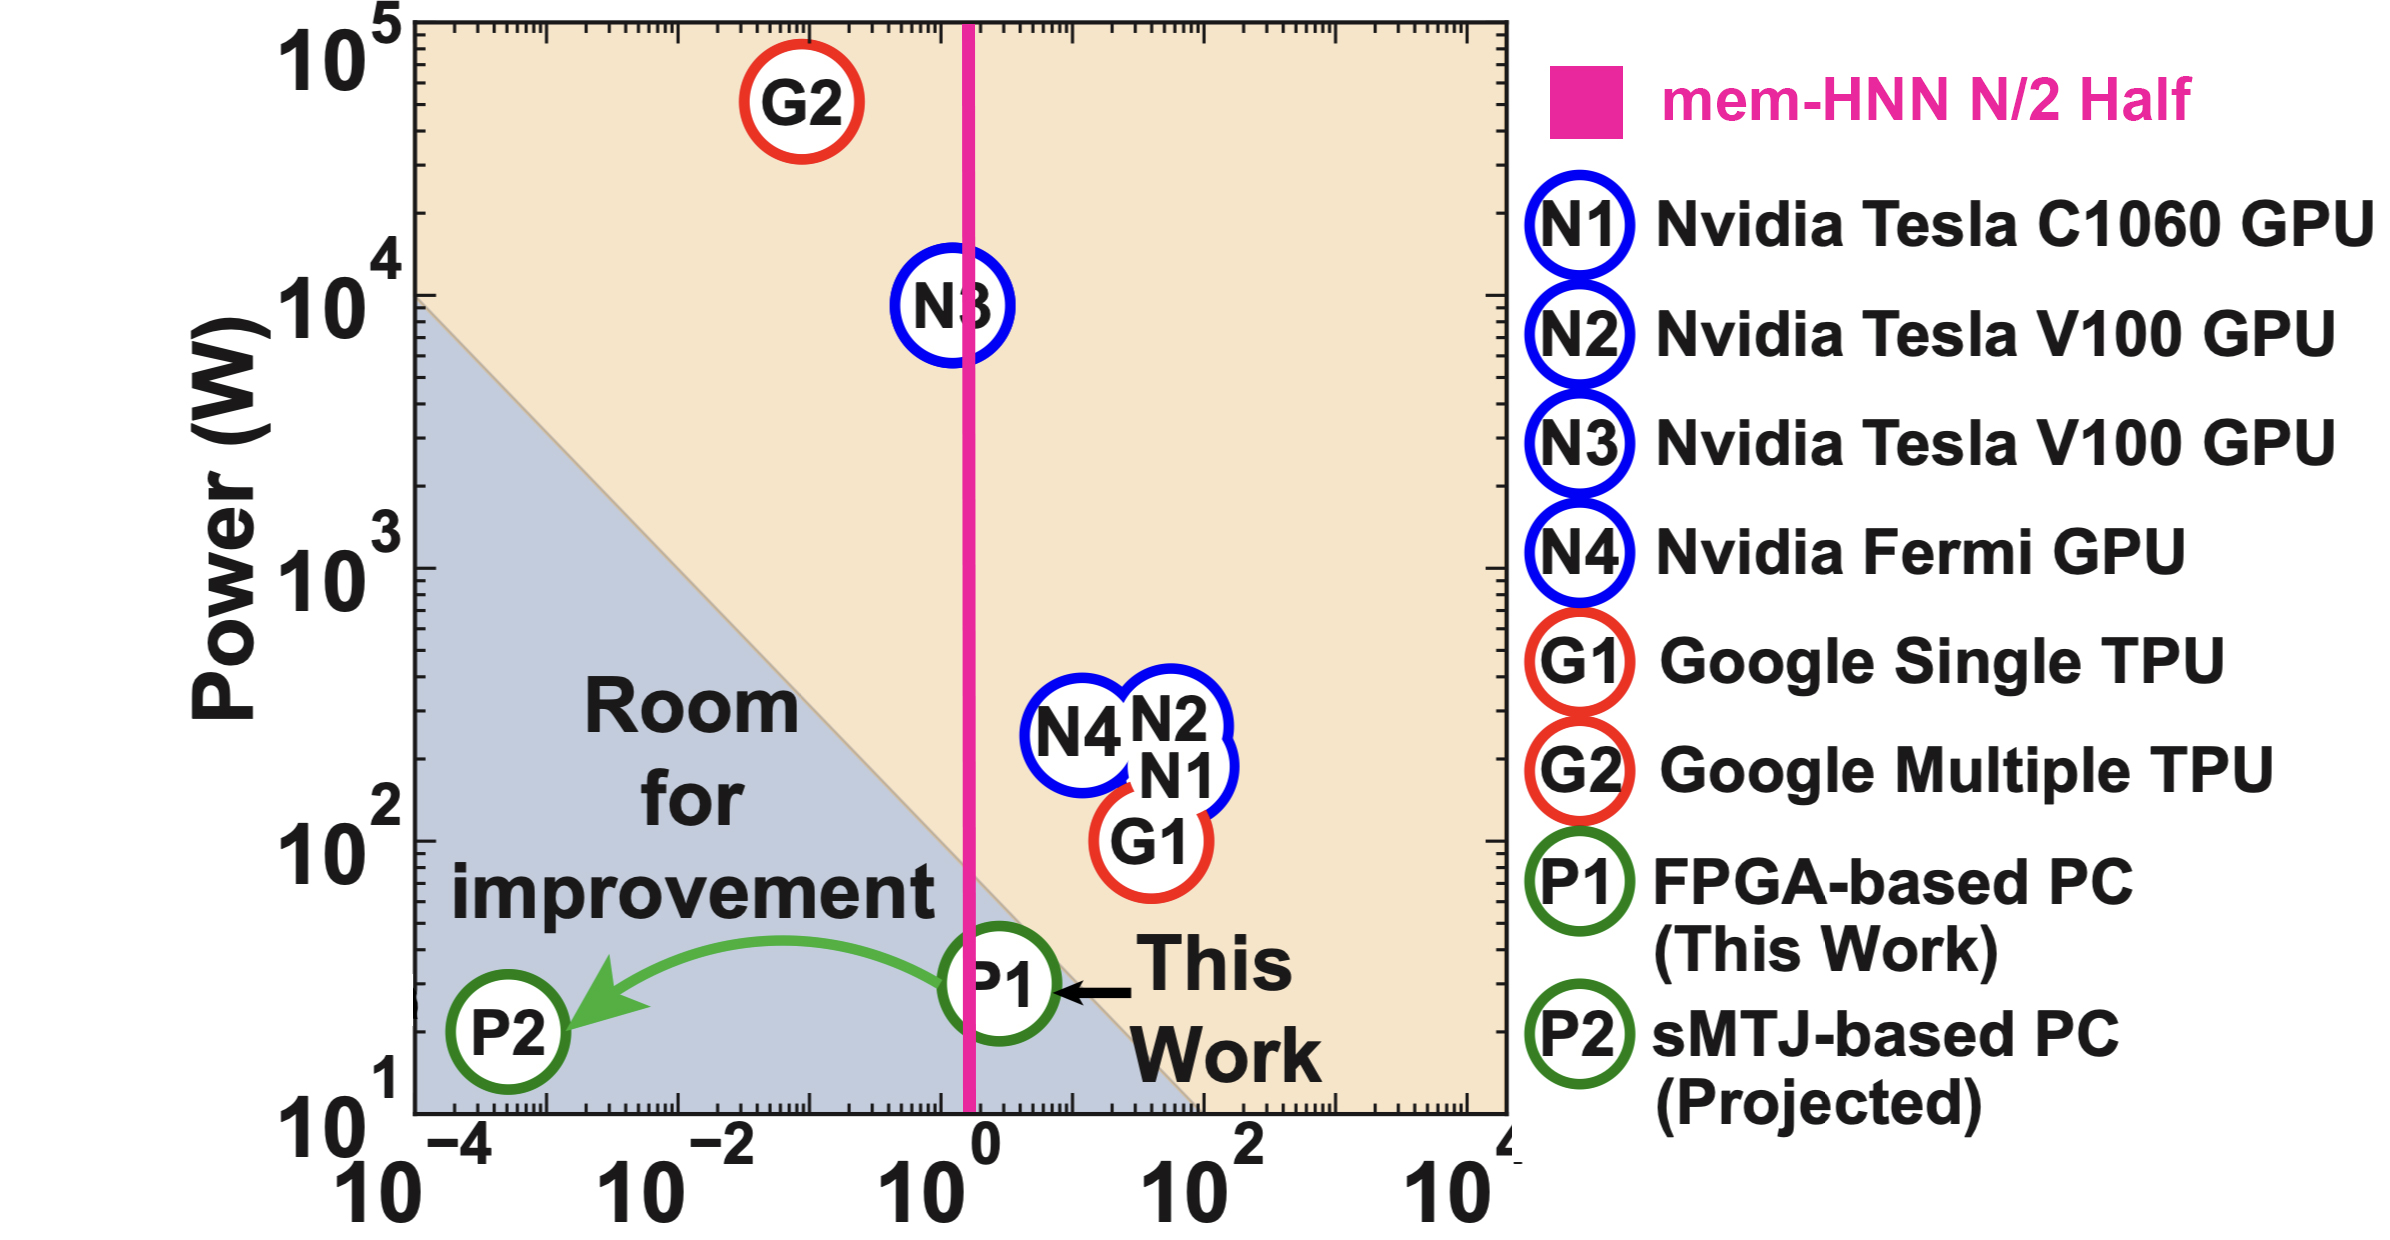
\includegraphics[width=0.9\linewidth]{graphics/Comparison_throughput_energy.jpg}
    \caption{Comparison throughput literature}
    \label{Comparison_throughput_literature}
\end{figure}

\section{Energy consumption}

Although the computation speed aligns with other probabilistic accelerators, the energy consumption here clearly sets it apart.
The resulsts show that the average sampling iteration requires beween 50 piko Joules and 20 piko Joules decreasing with ongoing training iterations.
Furthermore, to make these number comparable the power requiered is only \(\mathbf{22.5mW}\) decreasing over the training iterations to just under \(\mathbf{10mW}\).
This enables a complete training of the neural network with the consumption of only \(\mathbf{6 mJ}\) (720 Training iterations).
The training is simulated on a CPU\footnote{\texttt{Intel i7-10610U, 1.80GHz, 2304 Mhz, 4 Core(s), 8 Logical Processor(s)}}, which took 30minutes and has a thermal design power of 15W.
Therefore, the training used \textbf{27.000Joules}, which consumes \(\mathbf{460k \ x}\) more energy compared to the \ac{mem-HNN}.
For a complete comparison the energy consumption of the digital computer and the communication to the analog accelerator is not meassured 
would make the result worse. 
Compared to the listed NVIDIA \ac{GPU}s the power begins at \(\mathbf{10^2}\) reaching almost \(\mathbf{10^4}\) with one \ac{GPU},
which is by far worse than the proposed N/2 Half \ac{mem-HNN}. The closest comparison has a slightly faster time to sweep
but uses around \(\mathbf{10W}\), which is \(\mathbf{400x}\) worse than the \ac{mem-HNN}.\footcite[cf.][2]{aaditAcceleratingAdaptiveParallel2023}.
Since the aim is to achive new application for more sustainable AI models on this \ac{ASIC} accelerator, 
this can be seen as great achievement.

\section{diffusion}
Now that the results exist and have been processed, the diffusion phase of the \ac{DSR} framework 
requires that the results are generally made available to the public. 
The results and the implementation are handed over to HP Labs and are used as 
bases for further research.
The goal is to further develop the complete implementation of the model on the physical hardware accelerato.
Furhtermore, it is planned to take the results and add them to an upcoming paper that is presented
at TechCon, which is an HPE internal research fair. 
In addition to that, the results can be shown at public fairs that HPE plans on going in near future.
Lastly, this bachelor thesis is submitted to the DHBW-Stuttgart for assessment. 
